
In order to validate the good modeling of the main backgrounds
by the simulation, we
present here a first set of data to Monte Carlo comparisons in
control regions defined at the preselection level 
(see Section~\ref{sec:presel}), very far from the
signal regions that will be defined for the two analyses. We
are indeed interested in checking the data and backgrounds agreement
in selections free from eventual signal, and therefore a {\it blinding cut}
is defined using the $\htfj$ variable defined as the scalar sum of the
lepton transverse momentum, the first four leading jets transverse momenta
and the missing transverse energy. Considering the typical hardness of
\TTbar\ events, the region with $\htfj<800\gev$ can
safely be considered as signal-free. 
%It is worth noticing here that in the $\TTbar\to Wb+X$ analysis this cut is going to be inverted, obtaining an efficient reduction of background contributions, while in the  $\TTbar\to Ht+X$ analysis the  $H_T$ variable (with a slightly different definition, i.e. all jets are included in the sum and not only the first four) is going to be used to discriminate signal and background in the statistical analysis.
The preselection requirement of at least one \bjet\ enriches these control
regions in $\ttbar$+jets background, while  a selection vetoing \bjet s\
is considered to check the modeling of $W$+jets background.

Figure~\ref{fig:ELEMUON_4jetin1btagin} shows some kinematic distributions
comparing data and background prediction 
for the combined electron and muon channels,
requiring at least four jets and at least one \bjet\ 
in the signal-blind region  $\htfj<800\gev$. The \ttbar\ contribution 
is generated both with \texttt{MC@NLO} and \texttt{ALPGEN}, where the latter
is shown summed to the other background contributions and overlaid
as a dotted line.
A more complete set of plots, including the  \wjets\ enriched region, is available 
in Appendix~\ref{app:datamcpresel}. Yields for 
both selections are shown in Table~\ref{tab:yieldspresel} for electron
and muon channels combined. The yields for \ttbar\ predicted with \texttt{ALPGEN}
are $\sim$3-8\% higher than \texttt{MC@NLO}.
Looking at the distribution of the number of jets with $\pt>25\gev$
of Figure~\ref{fig:ELEMUON_4jetin1btaginNJETS} it is
evident that \texttt{ALPGEN} better models the high jet multiplicity
region. This is the main motivation for choosing to use \ttbar\ \texttt{ALPGEN}
samples in the \htx\ analysis, which requires at least six jets.
Tables for the electron and muon channels separately are available in  Appendix~\ref{app:datamcpresel}.

\begin{table}[htb]\centering
%        \resizebox{1.\textwidth}{!}{
        \begin{tabular}{l D{;}{\,\pm\,}{-1} D{;}{\,\pm\,}{-1} } \toprule\toprule
 & \multicolumn{1}{c}{ $\geq 4$ jets, $= 0$ $b$-tags } 		 & \multicolumn{1}{c}{ $\geq 4$ jets, $\geq 1$ $b$-tags } 		 \\ \midrule 
  MultiJet  & 15134;95  & 6264;74 \\ 
 Single top  & 3950;59  & 14375;107 \\ 
 Diboson  & 2172;22  & 548;12 \\ 
 $Z$+jets  & 31401;379  & 5804;146 \\ 
 $W$+jets  & 167551;947  & 35921;525 \\ 
 $t\bar{t}$V  & 113;1  & 680;2 \\ 
 $t\bar{t}$H (125)  & 24;0  & 220;1 \\ 
 $t\bar{t}$ MC@NLO  & 34563;131  & 202042;285 \\ 
\midrule 
  Tot Bkg w/ MC@NLO  & 254907;1034  & 265854;629 \\ \midrule 
  $T\bar{T}$ (600) chiral  & 3;1  & 36;2 \\ 
 Data  & 238709;489  & 256993;507 \\ 
\bottomrule\end{tabular}
%}
\caption{Yields for data, backgrounds and signal in the two blinded control
                regions with the ``preselection'' requirements but 
                with a veto on \btag ged jets
                (enriched in \wjets) and with at least one \btag ged jet
                (enriched in \ttbar). Uncertainties are only statistical.}\label{tab:yieldspresel}
\end{table}


\begin{figure}[htb]\begin{center}
	\subfigure[]{
  	\includegraphics[width=0.32\textwidth]{vlq_analysis/figures/THESIS_c5_presel_noortho_noyields/ELEMUON/4jetin/1btagin/LepPt_ELEMUON_4jetin1btagin_NOMINAL}}
	\subfigure[]{
  	\includegraphics[width=0.32\textwidth]{vlq_analysis/figures/THESIS_c5_presel_noortho_noyields/ELEMUON/4jetin/1btagin/LepEta_ELEMUON_4jetin1btagin_NOMINAL}}%\\
	\subfigure[]{
  	\includegraphics[width=0.32\textwidth]{vlq_analysis/figures/THESIS_c5_presel_noortho_noyields/ELEMUON/4jetin/1btagin/MET_ELEMUON_4jetin1btagin_NOMINAL}}
	\subfigure[]{
  	\includegraphics[width=0.32\textwidth]{vlq_analysis/figures/THESIS_c5_presel_noortho_noyields/ELEMUON/4jetin/1btagin/Wlep_MassT_ELEMUON_4jetin1btagin_NOMINAL}}
	\subfigure[]{
  	\includegraphics[width=0.32\textwidth]{vlq_analysis/figures/THESIS_c5_presel_noortho_noyields/ELEMUON/4jetin/1btagin/JetPt1_ELEMUON_4jetin1btagin_NOMINAL}}
	\subfigure[]{\label{fig:ELEMUON_4jetin1btaginNJETS}
  	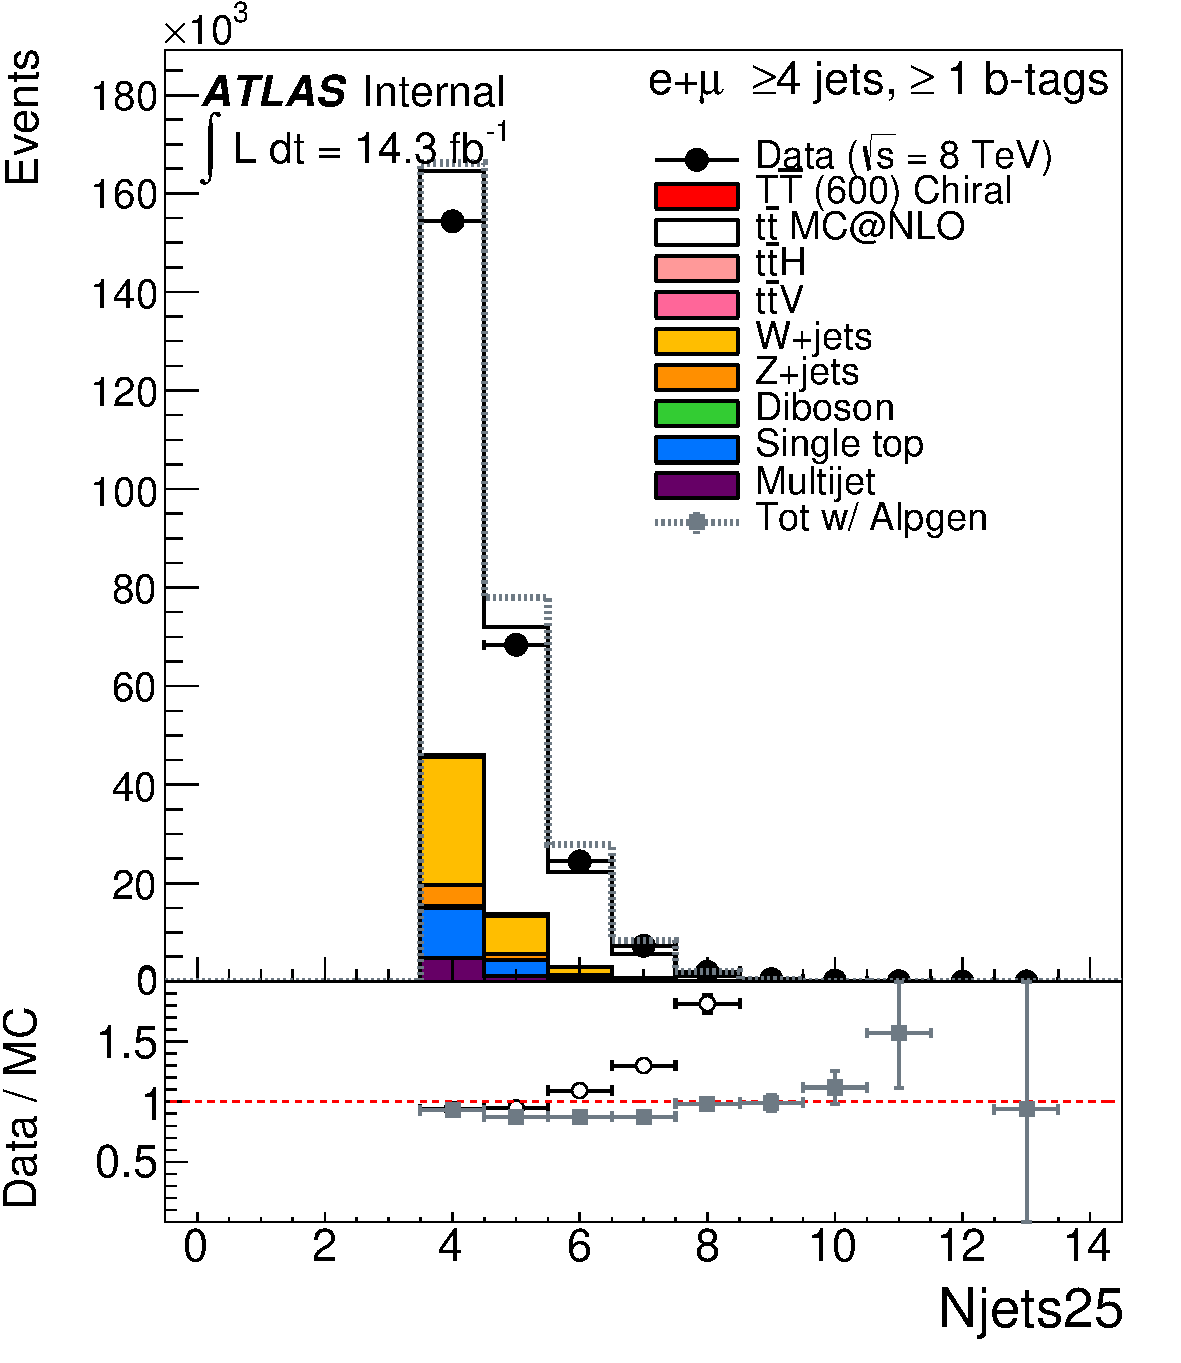
\includegraphics[width=0.32\textwidth]{vlq_analysis/figures/THESIS_c5_presel_noortho_noyields/ELEMUON/4jetin/1btagin/Njets25_ELEMUON_4jetin1btagin_NOMINAL}}
	%\subfigure[]{
  	%\includegraphics[width=0.32\textwidth]{vlq_analysis/figures/THESIS_c5_presel_noortho_noyields/ELEMUON/4jetin/1btagin/JetEta1_ELEMUON_4jetin1btagin_NOMINAL}}\\
	%\subfigure[]{
  	%\includegraphics[width=0.32\textwidth]{vlq_analysis/figures/THESIS_c5_presel_noortho_noyields/ELEMUON/4jetin/1btagin/nWhad_ELEMUON_4jetin1btagin_NOMINAL}}
	%\subfigure[]{
  	%\includegraphics[width=0.32\textwidth]{vlq_analysis/figures/THESIS_c5_presel_noortho_noyields/ELEMUON/4jetin/1btagin/Wlep_MassT_ELEMUON_4jetin1btagin_NOMINAL}}
	%\subfigure[]{
  	%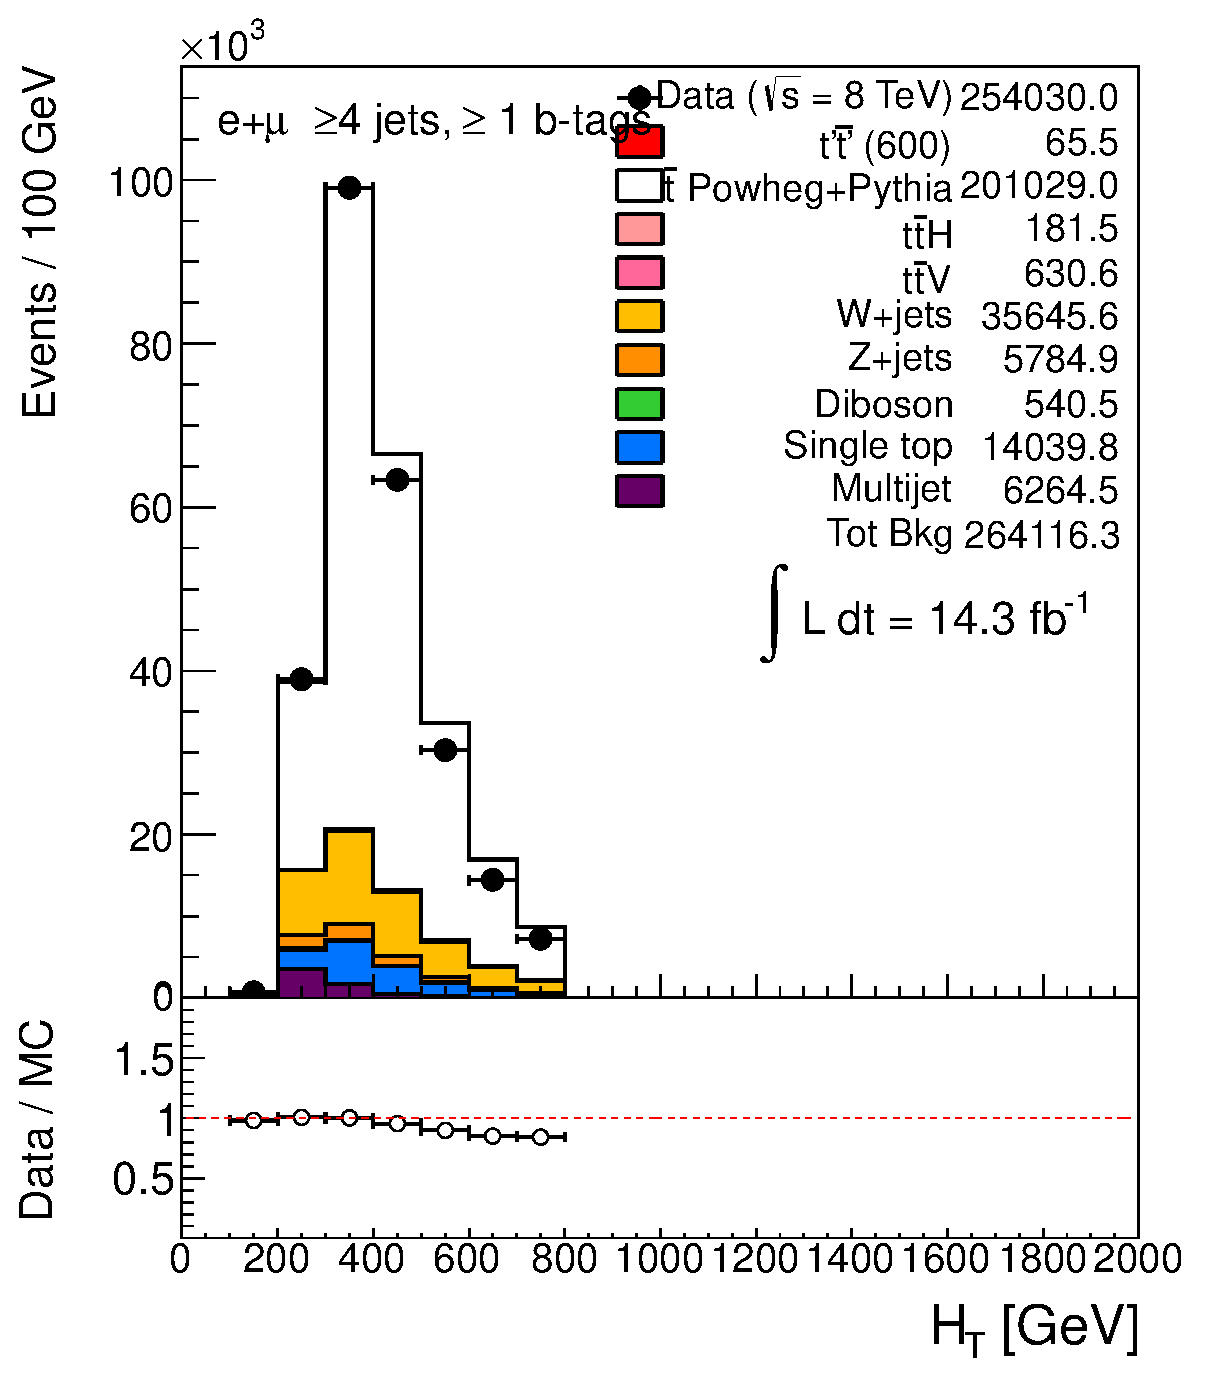
\includegraphics[width=0.32\textwidth]{vlq_analysis/figures/THESIS_c5_presel_noortho_noyields/ELEMUON/4jetin/1btagin/HTAll_ELEMUON_4jetin1btagin_NOMINAL}}
	\caption{Comparison between data and prediction plots for (a) lepton transverse momentum and
        (b) pseudorapidity, (c) missing tranverse energy, (d) transverse mass of $W$ boson, (e)
        leading jet transverse momentum, (f) number of jets with $\pt>25~\gev$.
        The selection is ``preselection'' with a blinding cut to reject signal on
        $\htfj<800\gev$. Systematic uncertainties are not shown.
        \label{fig:ELEMUON_4jetin1btagin}}
\end{center}\end{figure}
